\documentclass{beamer}
\mode<presentation> {
    \usetheme{Madrid}
    \usecolortheme{rose}
}
\usepackage{graphicx} 
\usepackage{booktabs} 
\usepackage[bookmarks=true]{hyperref}
\usepackage{caption}
\usepackage{amsmath} 
\captionsetup[figure]{labelformat=empty} 

\title[Attention Is All You Need]{Attention Is All You Need} 
\author{Yumeng Chu} 
\institute[NJUST] {Nanjing University of Science and Technology}
\date{ 2026} 

\begin{document}

\begin{frame}
    \titlepage 
\end{frame}

\begin{frame}{Contents}
    \tableofcontents
\end{frame}

\section{Introduction}
\begin{frame}{Introduction}
    \begin{itemize}
        \item \textbf{Background}: Dominant sequence transduction models (e.g., RNNs, LSTMs) rely on complex recurrent or convolutional neural networks.
        \item \textbf{Limitations}: 
        \begin{itemize}
            \item \textbf{RNNs}: Sequential nature precludes parallelization within training examples, hindering scalability for longer sequences.
            \item \textbf{CNNs}: Computational cost to relate signals from two distant positions grows with distance (linearly or logarithmically).
        \end{itemize}
        \item \textbf{Core Contribution}: Propose the \textbf{Transformer}, the first transduction model relying entirely on \textbf{Self-Attention} to compute input/output representations without recurrence or convolutions.
    \end{itemize}
\end{frame}

\section{Methodology}
\begin{frame}{Theoretical Framework: Scaled Dot-Product Attention}
    \begin{columns}[c] 
        \column{0.5\textwidth}
        \begin{center} % Centering the text and equation in this column
            \textbf{Attention Mechanism}
            \begin{equation*}
                \text{Attention}(Q,K,V) = \text{softmax}\left(\frac{QK^T}{\sqrt{d_k}}\right)V
            \end{equation*}
        \end{center}
        
        \begin{itemize}
            \item \textbf{Q, K, V}: Query, Key, and Value vectors.
            \item \textbf{Scaling Factor} $\frac{1}{\sqrt{d_k}}$: Prevents the dot product from growing too large.
            \item \textbf{Efficiency}: Optimized matrix multiplication.
        \end{itemize}
        
        \column{0.5\textwidth}
        \begin{figure}
            \centering
            
            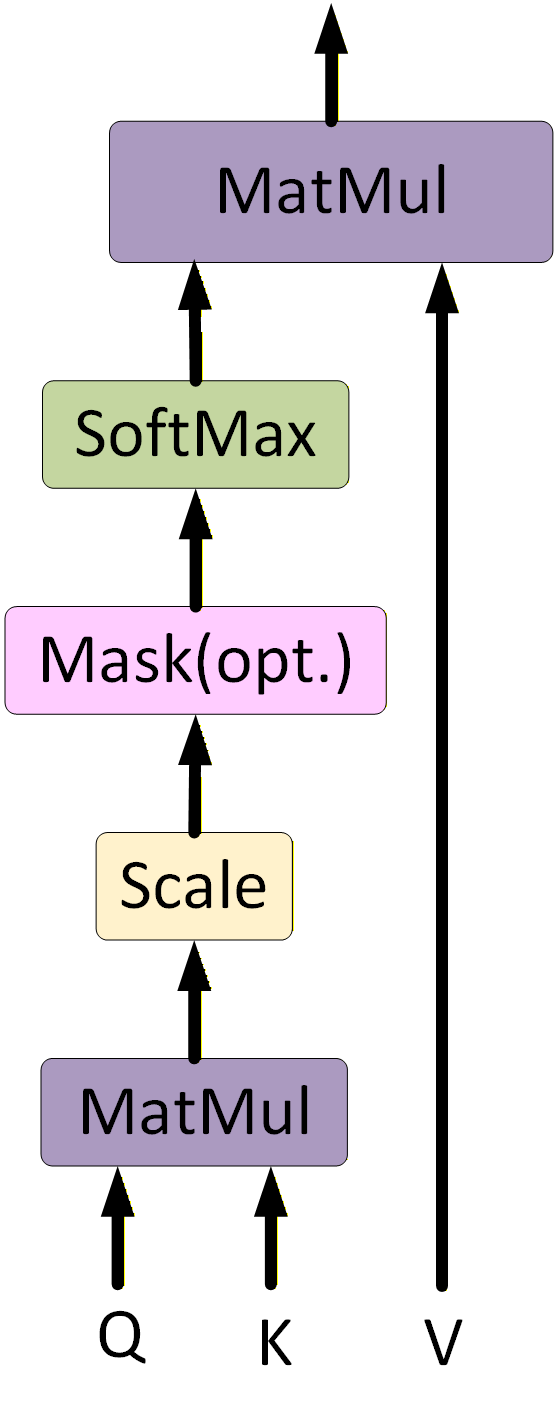
\includegraphics[width=0.4\linewidth,keepaspectratio]{Scaled_Dot-Product__Attention.png} 
            \caption{\footnotesize Fig 1: Scaled Dot-Product Attention}
        \end{figure}
    \end{columns}
\end{frame}

\begin{frame}{Theoretical Framework: Multi-Head Attention}
    \begin{itemize}
        \item \textbf{Concept}: Allows the model to jointly attend to information from different representation subspaces at different positions.
        \item \textbf{Mechanism}:
        \begin{equation*}
            \text{MultiHead}(Q,K,V) = \text{Concat}(\text{head}_1, ..., \text{head}_h)W^O
        \end{equation*}
        where $\text{head}_i = \text{Attention}(QW_i^Q, KW_i^K, VW_i^V)$.
        \item \textbf{Advantage}: Enables the model to capture complex semantic and syntactic dependencies in parallel.
    \end{itemize}
    \begin{center}
        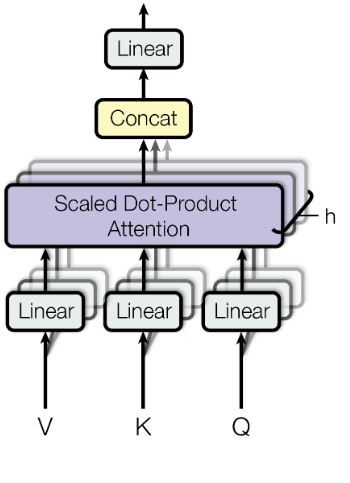
\includegraphics[height=0.4\textheight]{Multi-Head_Attention.png} 
    \end{center}
\end{frame}

\begin{frame}{Model Architecture}
    \begin{columns}[c]
        \column{0.4\textwidth}
        \begin{itemize}
            \item \textbf{Encoder-Decoder}: Stacked $N=6$ identical layers for both modules.
            \item \textbf{Residual Connections}: Applied to each sub-layer followed by Layer Normalization: $LayerNorm(x + Sublayer(x))$.
            \item \textbf{Positional Encoding}: Uses Sine/Cosine functions to inject information about the relative or absolute position of the tokens.
        \end{itemize}
        
        \column{0.6\textwidth}
        \begin{figure}
            \centering
            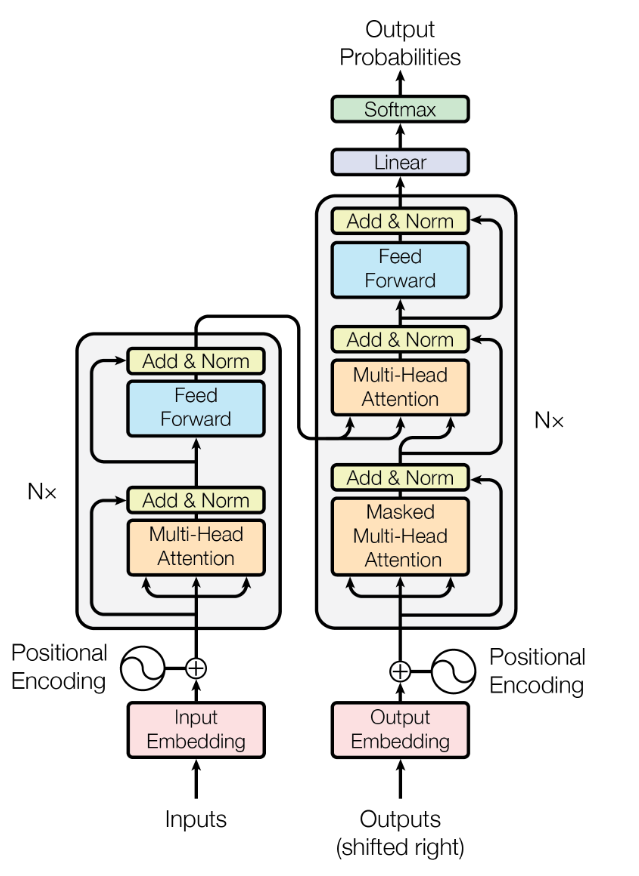
\includegraphics[height=0.75\textheight,keepaspectratio]{The_Transformer_model_architecture.png} 
            \caption{\footnotesize Fig 2: The Transformer Model Architecture}
        \end{figure}
    \end{columns}
\end{frame}

\section{Results}
\begin{frame}{Results: Performance \& Efficiency}
    \begin{itemize}
        \item \textbf{Translation Quality}: Achieves \textbf{28.4 BLEU} on WMT 2014 En-De, establishing a new state-of-the-art result.
        \item \textbf{Training Cost}: Significantly more parallelizable; reaches SOTA with a fraction of the training time compared to previous models.
    \end{itemize}
    \centering
    \vspace{0.2cm}
    \begin{table}[]
        \caption{Translation Performance and Training Cost}
        \resizebox{0.85\textwidth}{!}{
        \begin{tabular}{lccc}
            \toprule
            \textbf{Model} & \textbf{EN-DE (BLEU)} & \textbf{EN-FR (BLEU)} & \textbf{Training Cost (FLOPs)} \\
            \midrule
            ByteNet & 23.75 & - & $1.0 \times 10^{20}$ \\
            GNMT + RL & 24.6 & 39.92 & $2.3 \times 10^{19}$ \\
            \textbf{Transformer (base)} & 27.3 & 38.1 & $\mathbf{3.3 \times 10^{18}}$ \\
            \textbf{Transformer (big)} & \textbf{28.4} & \textbf{41.8} & $\mathbf{2.3 \times 10^{19}}$ \\
            \bottomrule
        \end{tabular}}
    \end{table}
\end{frame}

\section{Discussion}
\begin{frame}{Discussion: Self-Attention Visualizations}
    \begin{columns}[c]
        \column{0.5\textwidth}
        \begin{itemize}
            \item \textbf{Anaphora Resolution}: Different attention heads learn to resolve pronouns (e.g., "its") by attending to the correct nouns.
            \item \textbf{Syntactic Structure}: Model captures long-range dependencies, such as the relationship between a verb and its distant object.
        \end{itemize}
        
        \column{0.5\textwidth}
        \begin{figure}
            \centering
            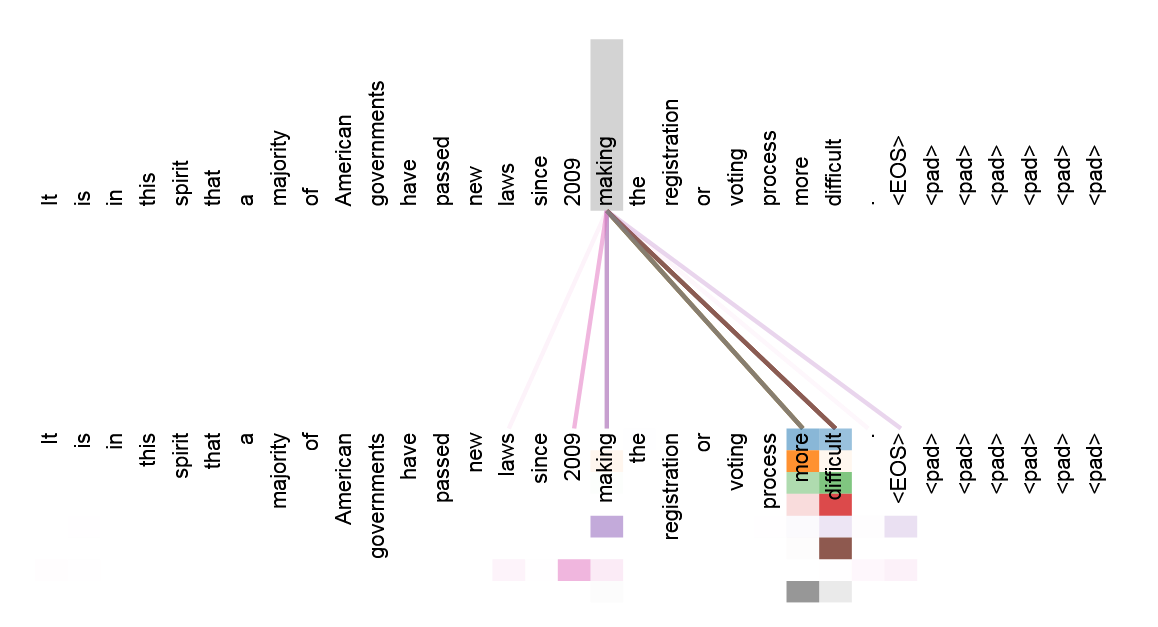
\includegraphics[width=\linewidth]{Attention_Visualization.png}
            \caption{\footnotesize Fig 3: Attention behavior for anaphora resolution}
        \end{figure}
    \end{columns}
\end{frame}

\section{Conclusion}
\begin{frame}{Conclusion}
    \begin{itemize}
        \item \textbf{Summary}: 
        \begin{enumerate}
            \item The Transformer is the first model to rely entirely on self-attention for sequence transduction.
            \item It achieves superior translation quality while being faster to train and more parallelizable.
        \end{enumerate}
        \item \textbf{Future Work}: 
        \begin{itemize}
            \item Applying Transformer to other modalities (e.g., images, audio).
            \item Investigating local, restricted attention mechanisms for very large inputs.
        \end{itemize}
    \end{itemize}
\end{frame}

\begin{frame}
    \centering
    \Huge{\textcolor[rgb]{0.7,0.1,0.1}{Thank you for your attention!}} \\
\end{frame}

\end{document}